\chapter{Комплекс функц, түүний хязгаар ба тасралтгүй чанар}
\section{Комплекс хувьсагчийн функц}
\begin{dfn}
$z\in D$ цэгт комплекс $w\in E$ тоо харгалзаж байх $f$ хууль өгөгдөж байвал $D\subset \overline{\mathbb{C}}$ олонлог дээр $f(z)$ функц өгөгдлөө гэх бөгөөд
\begin{equation}
f:D\rightarrow \overline{\mathbb{C}} \text{ буюу } w=f(z)
\end{equation}
тэмдэглэл хийдэг.

$D$ мужийг функцийн тодорхойлогдох,  $E$ мужийг өөрчлөгдөх муж гэж ярих ба $D$-г $\circled{z}$ хавтгайд $E$-г $\circled{w}$ хавтгайд авч заншжээ. Иймд, $w=f(z)$ функц $\circled{z}$ хавтгайн $D$ мужийг $\circled{w}$ хавтгайн $E$ мужид нэгэн утгатай буулгана. Энэ утгаар $w$-ийг $z$-ийн дүр, $z$-ийг эх дүр гэдэг.
\end{dfn}
\begin{exm}
$w=z^2$ функц I мөчийг хаана буулгах вэ?
\end{exm}
\begin{sol}
Эхлээд, $Oz$ цацрагийн дүр энэ буулгалтаар хаана гарахыг олъё.
\begin{center}
    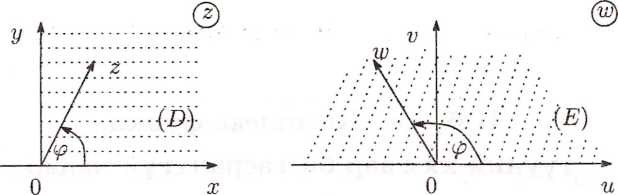
\includegraphics[width=9cm]{Zurag/4.jpg}
     \captionof{figure}{}
\end{center}
$\Arg  \varphi$ гэвэл $\Arg  w=\Arg(z^2)=2\cdot \Arg  x=2\varphi$ байх тул \\ $0\leq \varphi \leq \dfrac{\pi}{2}$ учир $0\leq \Arg  w \leq \pi$. Иймд $w=z^2$ функц I мөчийг дээд хагас хавтгайд буулгана. 
\end{sol}
$z=x+iy$, $w=u+iv$ гэвэл $f(z)=u(x,y)+iv(x,y)$ бичиглэл үйлдэж болно. Өөрөөр хэлбэл $z$ аргументийн комплекс\\ $w=f(z)$ функц нь хоёр хувьсагчийн $u(x,y)$, $v(x,y)$ хоёр функцээр тодорхойлогдох болж байна:
\begin{equation}
u(x,y)=\re f(z), v(x,y)=\im f(z)
\end{equation}
Дээрх $w=z^2$ функцийн бодит ба хуурмаг хэсгийг ол.
\begin{align*}
    &w=z^2=(x+iy)^2=x^2-y^2+2xyi \ \text{тул}\\
    &u(x,y)=\re (z^2)=x^2-y^2 \\
    &v(x,y) =\im (z^2)=2xy.
\end{align*}
\begin{hnt}
Хэрэв хоёр хувьсагчийн $u(x,y)$, $v(x,y)$ гэсэн хоёр функц $D(x,y)$ муж дээр өгөгдсөн гэвэл $w=u(x,y)+iv(x,y)$ нь комплекс $z=x+iy$ аргументийн комплекс функц байна.
\end{hnt}
\section{Функцийн хязгаар} \index{Функцийн хязгаар}
\begin{dfn}
    $z_0=(x_0,y_0)\in D$ байг. $w=f(z)$ нь $D\setminus\{z_0\}$ дээр тодорхойлогдсон функц байг. Хэрэв дараах нөхцөл хангах $A\in \mathbb{C}$ тоо олдож байвал $A$ тоог $w=f(z)$ функцийн $z\to z_0$ хязгаар гэнэ:
\begin{equation} \label{хязгаар тэмдэг}
    \forall \varepsilon >0 \ \  \exists \delta (\varepsilon, z_0)>0: 0<|z-z_0|<\delta \Rightarrow |f(x)-A|<\varepsilon 
    \end{equation}
$w=f(z)$ функцийн $z\to z_0$ хязгаарыг 
\begin{equation} \label{хязгаар}
\lim_{z\rightarrow z_0} f(z)=A
\end{equation}
гэж тэмдэглэнэ.
\end{dfn}
\begin{equation} \label{хязгаар}
\lim_{z\rightarrow z_0} f(z)=A=\alpha +i\beta
\end{equation}
 (\ref{хязгаар}) нь
\begin{equation}
\lim_{(x,y)\rightarrow (x_0,y_0)} u(x,y)=\alpha \qquad \lim_{(x,y)\rightarrow (x_0,y_0)} v(x,y)=\beta
\end{equation}
гэж хоёр хувьсагчийн хоёр функцийн хязгаар бодоход хүргэнэ. 

$z_0=\infty$ тохиолдолд функцийн хязгаар
$$\forall \varepsilon >0 \quad \exists R_0(\varepsilon): \quad |z|>R_0\Rightarrow |f(z)-A|<\varepsilon$$
гэж тодорхойлогдох бөгөөд
\begin{equation}
\lim_{z\rightarrow \infty} f(z)=A.
\end{equation}
\section{Функцийн хязгаар. Тасралтгүй чанар} \index{Тасралтгүй чанар}
Комплекс хувьсагчийн $w=f(z)$ функцийн $z_0\in D$ цэг дээр тасралтгүй байх нь
\begin{equation} \label{2.6}
\lim_{z\rightarrow z_0} f(z)=f(z_0)
\end{equation}
гэсэн хязгаарын тэнцлээр тодорхойлогдоно. Комплекс $z$ хувьсагчид $\Delta z=z-z_0$ өөрчлөлт өгвөл $w=f(z)$ функц харгалзан
$$\Delta w= \Delta f(z_0)=f(z)-f(z_0)$$
өөрчлөлт авч (\ref{2.6}) ёсоор
\begin{equation}
\lim_{\Delta z\rightarrow 0} \Delta w =0
\end{equation}
болж, өөрөөр хэлбэл аргументийн төгсгөлгүй бага өөрчлөлтөд функцийн төгсгөлгүй бага өөрчлөлт харгалзаж байвал\\ $w=f(z)$ функц $z_0$ цэг дээр тасралтгүй байна гэж ярьдаг.

Бид зөвхөн нэг утгат функцийн талаар авч үзлээ. Гэвч онолын болон олон тооны хавсарга ухаануудад олон хувьсагчийн комплекс функц авч үзэх шаардлага тулгардаг. Наад захын жишээ татахад л $\Arg  z$ функц байна. Энэ функц $z\neq 0$ утга бүхэнд нэг нь нөгөөгөөс $2\pi $ тоонд бүхлээр хуваагдах нэмэгдэхүүнээр ялгаатай төгсгөлгүй олон утга авна. Комплекс тооны язгуурын $w=\sqrt[n]{z}$ функц $n$ утгат функц болохтой өмнө танилцсан билээ. 

Нэг утгат тасралтгүй $w=f(z)$ функц $D\subset \mathbb{C}$ мужид тодорхойлогдсон байг. $\forall z_1\in D$, $\forall z_2\in D$ авахад $f(z_1)\neq f(z_2)$ байх нь зөвхөн $z_1\neq z_2$ байхад биелэгдэж байвал $f(z)$-ийг $D$ дээр харилцан нэг утгат буюу нэг хуудаст функц гэнэ.

Иймд, $w=f(z)$ нь $D$ мужид нэг хуудаст бөгөөд $D$-г $D^*$-д буулгах бол $D^*$ мужид урвуу $z=f^{-1}(w)$ функц оршин байх болов. Өөрөөр хэлбэл  $\forall z\in D$ хувьд $z=f^{-1}(f(z))$ ба $\forall w\in D^*$ хувьд $w=f(f^{-1}(w))$.
\section{Үндсэн элементар функцүүд}
Нэг утгат хялбар функцүүдийн нэг нь $w=z^n$, $n\in \mathbb{N}$ гэсэн зэрэгт функц. Зэрэгт функцийн тусламжтайгаар комплекс $z$ хувьсагчийн олон гишүүнт функц үүсгэнэ:
\begin{equation}
P_n(z)=a_0z^n+a_1z^{n-1}+\cdots +a_n, \qquad a_0\neq 0
\end{equation}
$a_0, \ldots , a_n$ коэффициентууд нь тогтмол комплекс тоонууд. Олон гишүүнт нь $\overline{\mathbb{C}}$ дээр тодорхойлогдоно. Энд $P_n(\infty)=\infty$ гэж үзнэ. Хялбар олон гишүүнт нь шугаман функц:
$$w=az+b, \quad a\neq 0.$$

Олон гишүүнтийг өөрөөр бүхэл рациональ функц гэнэ. Хоёр олон гишүүнтийн ноогдвороор бутархай рациональ $R(z) $ функц дүрслэгдэнэ:
\begin{equation}
R(z)=\dfrac{P_m(z)}{P_n(z)}=\dfrac{b_0z^m+b_1z^{m-1}+\cdots +b_m}{a_0z^n+a_1z^{n-1}+\cdots +a_n}, \quad a_0\neq 0
\end{equation}
Бутархай рационал хялбар
\begin{equation}
L(z)=\dfrac{az+b}{cz+d}, \quad
\begin{vmatrix}
a&b\\
c&d
\end{vmatrix}\neq 0
\end{equation}
функцийг бутархай шугаман буулгалт гэнэ. \\ $w=e^z$ \quad $(z=x+iy)$-ийг комплекс экспонент буюу илтгэгч функц \index{Илтгэгч функц}гэнэ. Энэ функц бодит илтгэгчийн бүхий л дүрэмд захирагдана. Харин комплекс хувьсагчийн илтгэгч функц үет функц байна. Учир нь
\begin{align*}
    e^{z+2n\pi i}&= e^{x+i(y+2n\pi)}=e^x[\cos (y+2n\pi)+i\sin (y+2n\pi)] \\
    &=e^x(\cos y+i\sin y)=e^{x+iy}=e^z
\end{align*}
болж $e^z$ нь $T=2n\pi i$ үет функц болох нь нотлогдов.

Эйлерийн томьёо ашиглаж тригонометр
\begin{equation}
\cos z=\dfrac{e^{iz}+e^{-iz}}{2}, \quad \sin z= \dfrac{e^{iz}-e^{-iz}}{2i}
\end{equation}
функцүүд $z\in\mathbb{C}$ дээр тодорхойлогдох бөгөөд
\begin{equation}
\tan z=\dfrac{\sin z}{\cos z}, \quad \cot z= \dfrac{\cos z}{\sin z}
\end{equation}
гэж тодорхойлогдох нь $\tan z$ нь $z_n=(2n+1)\dfrac{\pi}{2}$, $n=0, \pm 1, ...$ ба харин $\cot z$ нь $z_n=n\pi $ $(n=0, \pm 1,...)$ цэг дээр тодорхойлогдохгүй.

Гиперболлог синус, косинус функцүүд \index{Гиперболлог функцүүд } $\mathbb{C}$ хавтгайд
\begin{equation}
\sh z=\dfrac{e^z-e^{-z}}{2}, \quad \ch z= \dfrac{e^z+e^{-z}}{2}
\end{equation}
гэж тодорхойлогдох бөгөөд $\ch z =\cos iz$, $\sh z=-i\sin z$ байна. Комплекс аргументийн тригонометр мөн гиперболлог функцүүдийн хувьд бодит аргументийн эдгээр функцийн бүхий л чанар хадгалагдана.
$$\cos (z_1\pm z_2)=\cos z_1\cos z_2 \mp \sin z_1 \sin z_2$$
$$\sin (z_1\pm z_2)=\sin z_1\cos z_2 \pm \sin z_2 \cos z_1$$
томьёонууд ашиглаж тригонометр функцийн бодит ба хуурмаг хэсгийг олдог.
\begin{exm}
\begin{align*}
    \cos z&=\cos(x+iy)=\cos x\cos (iy)-\sin x \sin (iy) \\
    &= \cos x ch y -i\sin x \sh y =\cos x ch y -i\sin x \sh y
\end{align*}
байх тул  $$ \re (\cos z)= \cos x \ch y, \quad \im (\cos z)=-\sin x \sh y$$ болно. 
\end{exm}
Комплекс мужид илтгэгч функцийн урвуу функцийг логарифм функц \index{Логарифм функц} гэдэг. Өөрөөр хэлбэл хэрэв $w= ln z$ бол $z=e^w$ тэгшитгэлийг хангах $w$ олдоно: $w=u+iv$, $z=re^{i\varphi}=re^{i \Arg  z}$
гэж авбал 
$$z=re^{i \Arg  z}= e^{w}=e^u\cdot e^{iv}$$
бөгөөд эндээс $r=e^u$, $e^{i \Arg  z}=e^{iv}$ эхний тэгшитгэлээс $z\neq 0$ авбал $u=\ln r$ гэж нэг утгатай олдох ба харин дараах тэгшитгэлээс $u=\Arg  z$ гарна.

Иймд $z\neq 0$, $z\neq \infty$ байхад $w=\Ln z$ гэсэн олон утгат логарифм функц тодорхойлогдоно.
\begin{equation} \label{2.13}
w=\Ln z= \ln |z|+i (\arg  z+2n \pi), \quad n=0, \pm 1, ...
\end{equation}
(\ref{2.13})-аас $n=0$ тохиолдолд логарифмын гол утга гэж нэрлэгдэх
\begin{equation}
\ln z= \ln |z|+i \arg  z
\end{equation}
функц $\mathbb{C} \setminus \{ -\infty < x \leq 0, \quad y=0 \}$ өөрөөр хэлбэл $Ox$-ийн сөрөг чиглэлд хагалбартай бүх хавтгай муж дээр тасралтгүй, нэг утгатай байхаар оршин байна.

Тригонометр $\cos  z$, $\sin z$, $\tan z$-г функцүүдийн \index{Тригонометрийн урвуу функцүүд} хувьд тэдгээрийн урвуу болох $\Arccos z$, $\Arcsin z$, $\Arctan z$ зэрэг олон утгат функцүүд тодорхойлогдоно.
\begin{equation}
\Arccos z= -i \Ln (z+\sqrt{z^2-1}) 
\end{equation}
\begin{equation}
\Arcsin z= -i \Ln (iz-\sqrt{1-z^2}) 
\end{equation}
\begin{equation}
\Arctan z= -\dfrac{i}{2}\Ln \dfrac{1+iz}{1-iz}
\end{equation}
Мөн ерөнхий зэрэгт $z^a$, $a=\alpha +i\beta$  функц экспонентоор
\begin{equation}
z^a=e^{a\Ln z}
\end{equation}
ба гол утга нь
\begin{equation}
z^a=e^{a\ln z}
\end{equation}
гэж тодорхойлогдоно. Мөн ерөнхий илтгэгч $a^z$, $a\neq 0$ экспонентоор
\begin{equation}
a^z=e^{z\Ln a}
\end{equation}
ба гол утга нь
\begin{equation}
a^z=e^{z\ln a}
\end{equation}
\begin{exm}
$\cos (2+i)$ тооны бодит ба хуурмаг хэсгийг олъё.
\end{exm}
\begin{sol}
$\cos (2+i)=\cos 2\cdot \ch 1-i \sin 2\cdot \sh1$ тул $$\re \cos (2+i)=\cos 2 \sh1, \quad \im \cos (2+i)=-\sin 2\cdot \sh1$$
\end{sol}
\begin{exm}
Дараах утгуудыг бодож гарга.

\begin{enumerate}
\colgur{
    \item $\Ln (-1)$
    \item $ \Arccos \dfrac{1}{2}$
    \item $2^i$}
    \end{enumerate}
\end{exm}
\begin{sol}
\begin{enumerate}
    \item \begin{align*}
    \Ln(-1)&=\ln|-1|+i \arg  (-1)+2 k\pi i \\
    &= 0+\pi i +2 k \pi i= (2k+1)\pi i, \qquad k=0,\pm 1, ...
\end{align*}
\item 
\begin{align*}
    \Arccos\dfrac{1}{2}&= -i \Ln \left(\dfrac{1}{2}+\dfrac{\sqrt{3}}{2}i\right) \\
    &=-i \left(\ln\left|\dfrac{1}{2}+i\dfrac{\sqrt{3}}{2}\right|=\pm i\cdot \dfrac{\pi}{3}+2k\pi i\right)  \\
    &=2 k\pi \pm \dfrac{\pi}{3}
\end{align*}
\item 
\begin{align*}
    2^i&=e^{i \Ln 2} =e^{i(\ln|2|+0+2k\pi i)}=e^{i(\ln2+2k\pi i)}\\
    &=e^{-2k \pi} (\cos \ln 2+ i\sin \ln 2).
\end{align*}
\end{enumerate}
\end{sol}
\newpage
\begin{center}
    \textbf{Дасгал}
\end{center}
\begin{enumerate}
    \item [11.] Дараах илэрхийллийн бодит ба хуурмаг хэсгийг ол. \\
   \textbf{ 1.} $e^{z^2}$; \qquad \textbf{2. }$\ch (z-i)$; \qquad \textbf{3.} $\tan z$;
   \item [12.] Бодож гарга. \\
    \textbf{ 1.} $\Ln (-i)$; \qquad \textbf{2. }$\ln(-3-2i)$; \qquad \textbf{3.} $i^{\frac{1}{i}}$; \qquad \textbf{4.} $\left ( \dfrac{1+i}{\sqrt{2}}\right)2i$
    \item [13.] $\sin z=3$ тэгшитгэл бод.
    \item [14.] Алгебр хэлбэрт бич:\\
    \textbf{ 1.} $\sin \pi i$; \qquad \textbf{2. }$ \tan \dfrac{\pi}{2}i$; \qquad \textbf{3.} $\Arccos i$; \qquad \textbf{4.} $\Arctan \dfrac{i}{3}$;
\end{enumerate}